\documentclass{VUMIFPSkursinis}
\usepackage{algorithmicx}
\usepackage{algorithm}
\usepackage{algpseudocode}
\usepackage{amsfonts}
\usepackage{amsmath}
\usepackage{bm}
\usepackage{caption}
\usepackage{color}
\usepackage{float}
\usepackage{graphicx}
\usepackage{listings}
\usepackage{subfig}
\usepackage{wrapfig}
\usepackage{parcolumns}
\usepackage{enumitem}
%PAKEISTA, tarpai tarp sąrašo elementų
\setitemize{noitemsep,topsep=0pt,parsep=0pt,partopsep=0pt}
\setenumerate{noitemsep,topsep=0pt,parsep=0pt,partopsep=0pt}
\renewcommand{\lstlistingname}{Kodo ištrauka}

% Titulinio aprašas
\university{Vilniaus universitetas}
\faculty{Matematikos ir informatikos fakultetas}
\department{Programų sistemų katedra}
\papertype{Kursinis darbas}
\title{WebAssembly panaudojamumo galimybių analizė kuriant konkurencingas naujos kartos internetines programas }
\titleineng{WebAssembly Usability Analysis in Competitive Next-Generation Web Development}
\status{3 kurso 5 grupės studentas}
\author{Kasparas Taminskas}
\supervisor{Aurimas Šimkus}
\date{Vilnius – \the\year}

% Nustatymai
%\setmainfont{Palemonas}   % Pakeisti teksto šriftą į Palemonas (turi būti įdiegtas sistemoje)
\bibliography{bibliografija}

\begin{document}
	
% PAKEISTA	
\maketitle
\cleardoublepage\pagenumbering{arabic}
\setcounter{page}{2}

%TURINYS
\tableofcontents

\sectionnonum{Įvadas}
Interneto naudojimo reikšmė per 30 paskutiniųjų metų nuo žiniatinklio atsiradimo išaugo 
eksponentiškai. Nors saityno potencialas buvo pastebimas nuo pat pradžios, tačiau vargu, ar 
kas nors XX a. IX dešimtmetyje galėjo pagalvoti, jog auganti interneto reikšmė pasieks tokį 
lygį, jog tradicinės programų sistemos, turinčios didžiulę kodo bazę, kuriamos skirtingoms 
fizinėms platformoms ir programinėms aplinkoms, reikalaujančios intensyvaus mašininių resursų 
panaudojimo, bus taip pat pasiekiamos tiesiog vienu pelės paspaudimu, nepriklausys nuo 
konkrečios mašininės architektūros, programinės aplinkos ir nereikalaus jokių specialių 
diegimo etapų.

Šiomis dienomis programinės įrangos kūrimo rinkoje internetinės technologijos ir 
platformos, debesų kompiuterija yra įmonių dėmesio centre, nes galimybė pasiūlyti programinį 
produktą internetu atveria didelį konkurencinį pranašumą – klientams nebereikia įsidiegti 
programinės įrangos į savo elektroninius įrenginius, užtenka vienos programos – interneto 
naršyklės – kuri atveria plačias galimybes naudotis skirtingų tipų programomis, pateikiamomis, 
kaip paslauga klientui (angl. - Software as a Service). Be to, patys programų sistemų kūrėjai 
patiria mažesnius kaštus kurdami ir palaikydami savo produktus, nes nebelieka poreikio turėti 
skirtingų kodo bazių specifinėms operacinėms aplinkoms ar įrenginiams.

Poreikis turėti kompleksiškas programų sistemas internetinėje erdvėje kelia didelius 
reikalavimus pagrindiniams saityno technologijų kūrėjams – didiesiems naršyklių gamintojams – 
kurių technologiniai sprendimai įgalina programuotojus įgyvendinti programinius sprendimus 
internete: šios naujos kartos programos internete turi užtikrinti tokius pačius kokybinius 
reikalavimus - greitaveiką, saugumą ir patikimumą - kaip senosios. Šioje vietoje susiduriama 
su dideliais technologiniais naršyklių variklių implementacijos ir pagrindinės internetinių 
technologijų programinės kalbos – JavaScript – ribojimais, neleidžiančiais įgyvendinti 
internetinių programų visiško supanašėjimo su tradicinėmis, veikiančiomis specifinėse 
platformose. 

WebAssembly standarto specfikacija ir jos formalus įgyvendinimas naršyklių 
smėliadėžės (angl. – sandbox) aplinkose siūlo sprendimą – binarinio formato kodo vykdymą 
greitaveikai imliose programų sistemų verslo logikos vietose papildant tradicinį JavaScript 
kodą. Ši technologinė naujovė, apibrėžta Pasaulinio žiniatinklio konsorciumo (W3C) ir palaikoma
visų modernių naršyklių kūrėjų, leidžia ženkliai sumažinti likusius techninius barjerus tarp 
naujos kartos internetinių programų sistemų ir tradicinių, nuo vykdymo aplinkos priklausamų 
sprendimų, todėl atveria saityne dar neišnaudotas rinkos perspektyvas, sėkmingai gyvuojančias
tradicinėse platformose. 

Šio darbo tikslas – pasiūlyti konkrečius variantus, kaip standartas 
gali būti integruotas į naujus ir jau egzistuojančius internetinius programinius sprendimus. 
Šie būdai leis programų sistemų kūrėjams išnaudoti stipriąsias technologijos dalis ir taip 
įgauti didesnį konkurencinį pranašumą internetinėje programų sistemų rinkoje.

\section{Žiniatinklio ekosistemos technologinė raida}

Siekiant geriau suprasti dabartinę padėtį, kurioje buvo pristatytas WebAssembly standartas ir kokius poreikius jis patenkina, yra būtina apžvelgti viso žiniatinklio populiarumo augimą ir jo technologinę raidą.

\subsection{Interneto populiarumo augimas}

Interneto bendruomenę sudarančių žemės gyventojų skaičius šiuo metu viršija pusę visos Žemės populiacijos. Šis augimas, prasidėjęs 1995 metais, kai Saitynas atsivėrė plačiai pasaulio bendruomenei, nestoja ir toliau, tą galima pastebėti iš \ref{fig:internet_usage} paveikslėlyje matomos viešos metinės statistikos. 

\begin{figure}[h!]
  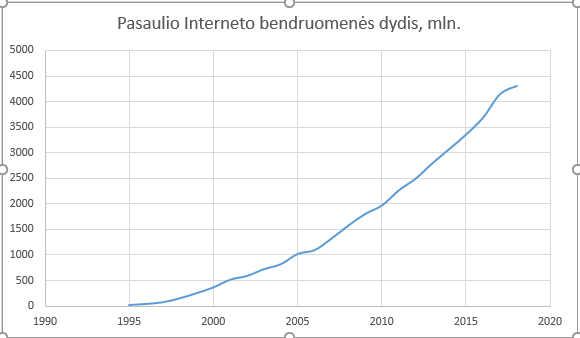
\includegraphics[scale=1]{interneto_naudojimo_statistika.png}
  \caption{Interneto bendruomenės narių skaičius 1995-2018}
  \label{fig:internet_usage}
\end{figure}

Ši statistika tik patvirtina plataus Interneto technologijų pritaikymo poreikio aktualumą ir didelę atsakomybę, tenkančią šių technologijų vedliams - interneto naršyklių kūrėjams. Žiniatinklis jau seniai nėra skirtas tik informacijos paieškai ir dalinimuisi, ką įgalino pradinės saityno technologijos - HTTP protokolas, HTML ir CSS žymėjimo kalbos. Šiuo metu vis didesnį pagreitį įgauna virtualios realybės, žaidimų industrijos, filmų ir muzikos sferų, neuroninių tinklų kūrimo ir analizės įrankiai. Deja, bet dažnai šių sprendimų pasiūlymas Internete būna ribotas dėl fundamentalių architektūrinių principų, kuriais paremtas programinio kodo vykdymas interneto naršyklėse.

\subsection{Programinio kodo vykdymas naršyklėse}
Interneto naršyklė architektūriniu požiūriu yra itin sudėtinga programa, nes procese nuo resurso parsiuntimo iš nutolusio serverio iki jo grafinio atvaizdavimo naršyklės lange dalyvauja daug sisteminių programos komponentų, nurodytų \ref{fig:browser_architecture} paveikslėlyje. 

\begin{figure}[h!]
  \begin{center}
  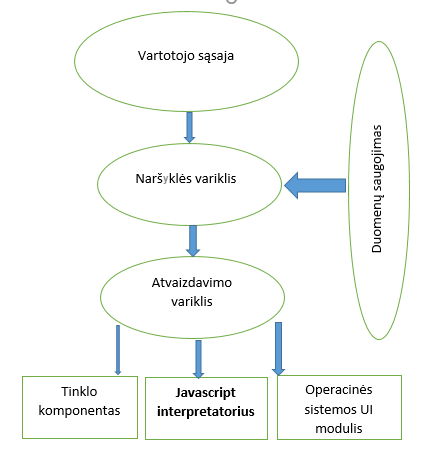
\includegraphics[scale=0.8]{naršyklės_architektūra.png}
  \end{center}
  \caption{Aukšto lygio interneto naršyklės veikimo principas}
  \label{fig:browser_architecture}
\end{figure}

Vienas esminių šios schemos komponentų - Javascript interpretatorius - žiniatinkliui suteikia dinamiškumą ir leidžia vykdyti skriptus, parašytus Javascript programavimo kalba, tiesiog naršyklėje. Interpretatoriaus rezultatai siunčiami atvaizdavimo varikliui, kuris pasirūpina jų išdėstymu interneto aplikacijoje.

\subsubsection{JavaScript kalbos savybės}

Nuo pat žiniatinklio atsiradimo pradžios interneto technologijų branduolį sudaro Javascript programavimo kalba, kurios prototipas per 10 dienų buvo sukurtas 1995 metais kompanijos Netscape Communications. Ši programavimo kalba žiniatinklyje iki šiol užėmė visišką monopoliją, interneto aplikacijų klientinės dalies kūrimas be jos yra tiesiog sunkiai įsivaizduojamas atvejis. Kalbos populiarumą ir išplitimą patvirtina GitHub saugyklos repozitorijų statistiniai duomenys, pagal kuriuos kalba jau ilgą laiką pirmauja turėdama virš 320000 aktyvių repozitorijų. 

\subsubsubsection{Dinaminė prigimtis}

Javascript programavimo kalba pasižymi dinaminiais tipais, t.y. kintamieji savo reikšmių tipus gali keisti skripto vykdymo metu. Žemiau pateikta \ref{lst:javascript_dinamiskumas} kodo ištrauka yra visiškai validi ir leidžiama interpretatoriaus.

\begin{center}
\begin{tabular}{c}
\begin{lstlisting}[caption={Dinaminiai tipai JavaScript kalboje}\label{lst:javascript_dinamiskumas}]
var x = 10;                   //console.log(x) => 10
x = "sveiki";                 //console.log(x) => sveiki
x = {                         //console.log(x) => [Object]
    a: "sveiki is objekto",
    b: 10,
    c: true
}
\end{lstlisting}
\end{tabular}
\end{center}

Ši kalbos savybė leidžia programuotojams savo kodo vykdymo rezultatus stebėti itin greitai, būtent dėl to interneto technologijų bendruomenė taip ją pamėgo

\subsubsection{Interpretavimo ir kompiliavimo skirtumai}

\subsubsection{Skirsnis}
\subsubsubsection{Straipsnis}
\subsubsection{Skirsnis}
\section{Skyrius}
\subsection{Poskyris}
\subsection{Poskyris}

\sectionnonum{Rezultatai ir išvados}
Rezultatų ir išvadų dalyje turi būti aiškiai išdėstomi pagrindiniai darbo
rezultatai (kažkas išanalizuota, kažkas sukurta, kažkas įdiegta) ir pateikiamos
išvados (daromi nagrinėtų problemų sprendimo metodų palyginimai, teikiamos
rekomendacijos, akcentuojamos naujovės).


%% PAKEISTAS PAVADINIMAS Į 'Šaltiniai'
\printbibliography[heading=bibintoc, title=Šaltiniai]  % Šaltinių sąraše nurodoma panaudota
% literatūra, kitokie šaltiniai. Abėcėlės tvarka išdėstomi darbe panaudotų
% (cituotų, perfrazuotų ar bent paminėtų) mokslo leidinių, kitokių publikacijų
% bibliografiniai aprašai.  Šaltinių sąrašas spausdinamas iš naujo puslapio.
% Aprašai pateikiami netransliteruoti. Šaltinių sąraše negali būti tokių
% šaltinių, kurie nebuvo paminėti tekste.

% \sectionnonum{Sąvokų apibrėžimai}
\sectionnonum{Santrumpos}
Sąvokų apibrėžimai ir santrumpų sąrašas sudaromas tada, kai darbo tekste
vartojami specialūs paaiškinimo reikalaujantys terminai ir rečiau sutinkamos
santrumpos.

\appendix  % Priedai
% Prieduose gali būti pateikiama pagalbinė, ypač darbo autoriaus savarankiškai
% parengta, medžiaga. Savarankiški priedai gali būti pateikiami ir
% kompaktiniame diske. Priedai taip pat numeruojami ir vadinami. Darbo tekstas
% su priedais susiejamas nuorodomis.

\section{Neuroninio tinklo struktūra}
\begin{figure}[H]
    \centering
    \includegraphics[scale=0.5]{img/MLP}
    \caption{Paveikslėlio pavyzdys}
    \label{img:mlp}
\end{figure}


\section{Eksperimentinio palyginimo rezultatai}
% tablesgenerator.com - converts calculators (e.g. excel) tables to LaTeX
\begin{table}[H]\footnotesize
  \centering
  \caption{Lentelės pavyzdys}
  {\begin{tabular}{|l|c|c|} \hline
    Algoritmas & $\bar{x}$ & $\sigma^{2}$ \\
    \hline
    Algoritmas A  & 1.6335    & 0.5584       \\
    Algoritmas B  & 1.7395    & 0.5647       \\
    \hline
  \end{tabular}}
  \label{tab:table example}
\end{table}

\end{document}
